\documentclass[review]{elsarticle}
\usepackage{subfig}
\usepackage{float} %Permite manejar/mover/partir mejor figuras y tablas
\usepackage{lineno,hyperref}
\usepackage{eurosym}
\modulolinenumbers[5]

\journal{Spectrochimica Acta, Part B: Atomic Spectroscopy}

%%%%%%%%%%%%%%%%%%%%%%%
%% Elsevier bibliography styles
%%%%%%%%%%%%%%%%%%%%%%%
%% To change the style, put a % in front of the second line of the current style and
%% remove the % from the second line of the style you would like to use.
%%%%%%%%%%%%%%%%%%%%%%%

%% Numbered
%\bibliographystyle{model1-num-names}

%% Numbered without titles
%\bibliographystyle{model1a-num-names}

%% Harvard
%\bibliographystyle{model2-names.bst}\biboptions{authoryear}

%% Vancouver numbered
%\usepackage{numcompress}\bibliographystyle{model3-num-names}

%% Vancouver name/year
%\usepackage{numcompress}\bibliographystyle{model4-names}\biboptions{authoryear}

%% APA style
%\bibliographystyle{model5-names}\biboptions{authoryear}

%% AMA style
%\usepackage{numcompress}\bibliographystyle{model6-num-names}

%% `Elsevier LaTeX' style
\bibliographystyle{elsarticle-num}
%%%%%%%%%%%%%%%%%%%%%%%

\begin{document}

\begin{frontmatter}

\title{PETALO, a positron emission TOF apparatus using liquid xenon}
%\tnotetext[mytitlenote]{Fully documented templates are available in the elsarticle package on \href{http://www.ctan.org/tex-archive/macros/latex/contrib/elsarticle}{CTAN}.}

%% Group authors per affiliation:
\author{J.J. Gomez-Cadenas, J.M. Benlloch Rodriguez and Paola Ferrario}
\address{IFIC (U. Valencia/CSIC)}
%\fntext[myfootnote]{Since 1880.}

%% or include affiliations in footnotes:
%\author[mymainaddress,mysecondaryaddress]{Elsevier Inc}
%\ead[url]{www.elsevier.com}
%
%\author[mysecondaryaddress]{Global Customer Service\corref{mycorrespondingauthor}}
%\cortext[mycorrespondingauthor]{Corresponding author}
%\ead{support@elsevier.com}
%
%\address[mymainaddress]{1600 John F Kennedy Boulevard, Philadelphia}
%\address[mysecondaryaddress]{360 Park Avenue South, New York}

\begin{abstract}
We describe a new Positron Emission TOF Apparatus using Liquid xenOn (PETALO). The detector is based in the Liquid Xenon Scintillating Cell (LXSC). The cell shape and dimensions  can be optimised depending on the intended application. In its simplest form, the LXSC is a box in which two faces are covered by SiPMs and the others by a reflecting material such as Teflon. The LXSC is a compact, homogenous and highly efficient detector which shares many of the desirable properties of monolithic crystals, with the added advantage of high yield and fast scintillation offered by liquid xenon. Our initial studies suggest that good energy and spatial resolution comparable with that achieved by LYSO crystals can be obtained with a detector based in LXSCs. In addition, the system can potentially achieve an excellent coincidence resolution time (CRT) of better than 100 ps. 
\end{abstract}

\begin{keyword}
PET \sep TOF \sep Liquid Xenon \sep energy resolution \sep
 high sensitivity \sep coincidence resolution time (CRT) \sep SiPMs.
\end{keyword}

\end{frontmatter}

%\linenumbers
% BB
\newcommand{\bb}{\ensuremath{\beta\beta}}
% BB0NU
\newcommand{\bbonu}{\ensuremath{\beta\beta0\nu}}
% BB2NU
\newcommand{\bbtnu}{\ensuremath{\beta\beta2\nu}}
% NME
\newcommand{\Monu}{\ensuremath{\Big|M_{0\nu}\Big|}}
\newcommand{\Mtnu}{\ensuremath{\Big|M_{2\nu}\Big|}}
% PHASE-SPACE FACTOR
\newcommand{\Gonu}{\ensuremath{G_{0\nu}(\Qbb, Z)}}
\newcommand{\Gtnu}{\ensuremath{G_{2\nu}(\Qbb, Z)}}

% mbb
\newcommand{\mbb}{\ensuremath{m_{\beta\beta}}}
\newcommand{\kgy}{\ensuremath{\rm kg \cdot y}}
\newcommand{\ckky}{\ensuremath{\rm counts/(keV \cdot kg \cdot yr)}}
\newcommand{\mbba}{\ensuremath{m_{\beta\beta}^a}}
\newcommand{\mbbb}{\ensuremath{m_{\beta\beta}^b}}
\newcommand{\mbbt}{\ensuremath{m_{\beta\beta}^t}}
\newcommand{\nbb}{\ensuremath{N_{\beta\beta^{0\nu}}}}

% Qbb
\newcommand{\Qbb}{\ensuremath{Q_{\beta\beta}}}

% Tonu
\newcommand{\Tonu}{\ensuremath{T_{1/2}^{0\nu}}}

% Tonu
\newcommand{\Ttnu}{\ensuremath{T_{1/2}^{2\nu}}}

% Xe-136
\newcommand{\Xe}{\ensuremath{^{136}}Xe}
\newcommand{\COT}{\ensuremath{CO_2}}
\newcommand{\CHF}{\ensuremath{CH_4}}
\newcommand{\CFF}{\ensuremath{CF_4}}

% 2S
\newcommand{\TwoS}{\ensuremath{^{2}S_{1/2}}}

\newcommand{\TwoP}{\ensuremath{^{2}P_{1/2}}}

\newcommand{\TwoD}{\ensuremath{^{2}D_{3/2}}}


% Xe-136
\newcommand{\CS}{\ensuremath{^{137}}Cs}

% Xe-136
\newcommand{\NA}{\ensuremath{^{22}}Na}


% Bi-214
\newcommand{\Bi}{\ensuremath{^{214}}Bi}

% Tl-208
\newcommand{\Tl}{\ensuremath{^{208}}Tl}

% Pb-208
\newcommand{\Pb}{\ensuremath{^{208}}Pb}
% Pb-208
\newcommand{\PBD}{\ensuremath{^{210}}Pb}

% Po-214
\newcommand{\Po}{\ensuremath{^{214}}Po}
\newcommand{\Kr}{\ensuremath{^{83}}Kr}

% bru
\newcommand{\bru}{cts/(keV$\cdot$kg$\cdot$y)}
\newcommand{\dten}{10 mm/$\sqrt{\rm m}$}
\newcommand{\dtwo}{2 mm/$\sqrt{\rm m}$}
\newcommand{\BAPP}{\ensuremath{Ba^{++}}}
\newcommand{\BAP}{\ensuremath{Ba^{+}}}

\newcommand{\HPXE}{\sc{HPXe}\rm}
\newcommand{\BATA}{\sc{BaTa}\rm}

% Saltos de carro en tablas
\newcommand{\minitab}[2][l]{\begin{tabular}{#1}#2\end{tabular}}

\newcommand{\thedraft}{0.1.1}% version for referees

\newcommand{\MO}{\ensuremath{{}^{100}{\rm Mo}}}
\newcommand{\SE}{\ensuremath{{}^{82}{\rm Se}}}
\newcommand{\ZR}{\ensuremath{{}^{96}{\rm Zr}}}
\newcommand{\KR}{\ensuremath{{}^{82}{\rm Kr}}}
\newcommand{\ND}{\ensuremath{{}^{150}{\rm Nd}}}
\newcommand{\XE}{\ensuremath{{}^{136}\rm Xe}}
\newcommand{\GE}{\ensuremath{{}^{76}\rm Ge}}
\newcommand{\GES}{\ensuremath{{}^{68}\rm Ge}}
\newcommand{\TE}{\ensuremath{{}^{128}\rm Te}}
\newcommand{\TEX}{\ensuremath{{}^{130}\rm Te}}
\newcommand{\TL}{\ensuremath{{}^{208}\rm{Tl}}}
\newcommand{\CA}{\ensuremath{{}^{48}\rm Ca}}
\newcommand{\CO}{\ensuremath{{}^{60}\rm Co}}
\newcommand{\PO}{\ensuremath{{}^{214\rm Po}}}
\newcommand{\U}{\ensuremath{{}^{235}\rm U}}
\newcommand{\CT}{\ensuremath{{}^{10}\rm C}}
\newcommand{\BE}{\ensuremath{{}^{11}\rm Be}}
\newcommand{\BO}{\ensuremath{{}^{8}\rm Be}}
\newcommand{\UDTO}{\ensuremath{{}^{238}\rm U}}
\newcommand{\CD}{\ensuremath{^{116}{\rm Cd}}}
\newcommand{\THO}{\ensuremath{{}^{232}{\rm Th}}}
\newcommand{\BI}{\ensuremath{{}^{214}}Bi}
\newcommand{\FDG}{\ensuremath{^{18}}F}


\section{Introduction}

Positron Emission Tomography (PET) is a non invasive imaging technique that produces a three-dimensional image of functional processes --it does not show anatomic features, but it rather  measures the metabolic activity of the cells-- in the body. PET is used in
both clinical and pre-clinical research to study the molecular bases and treatments of
disease. In clinical applications, PET has proven its critical value in several areas such as
cancer diagnosing and staging, assessing neurological diseases such as Alzheimer's disease
and dementias, myocardium blood flow and viability evaluation in cardiology, as well as an
increasing role in radiotherapy treatment planning and chemotherapy monitoring. 

\begin{figure}[!htb]
	\centering
	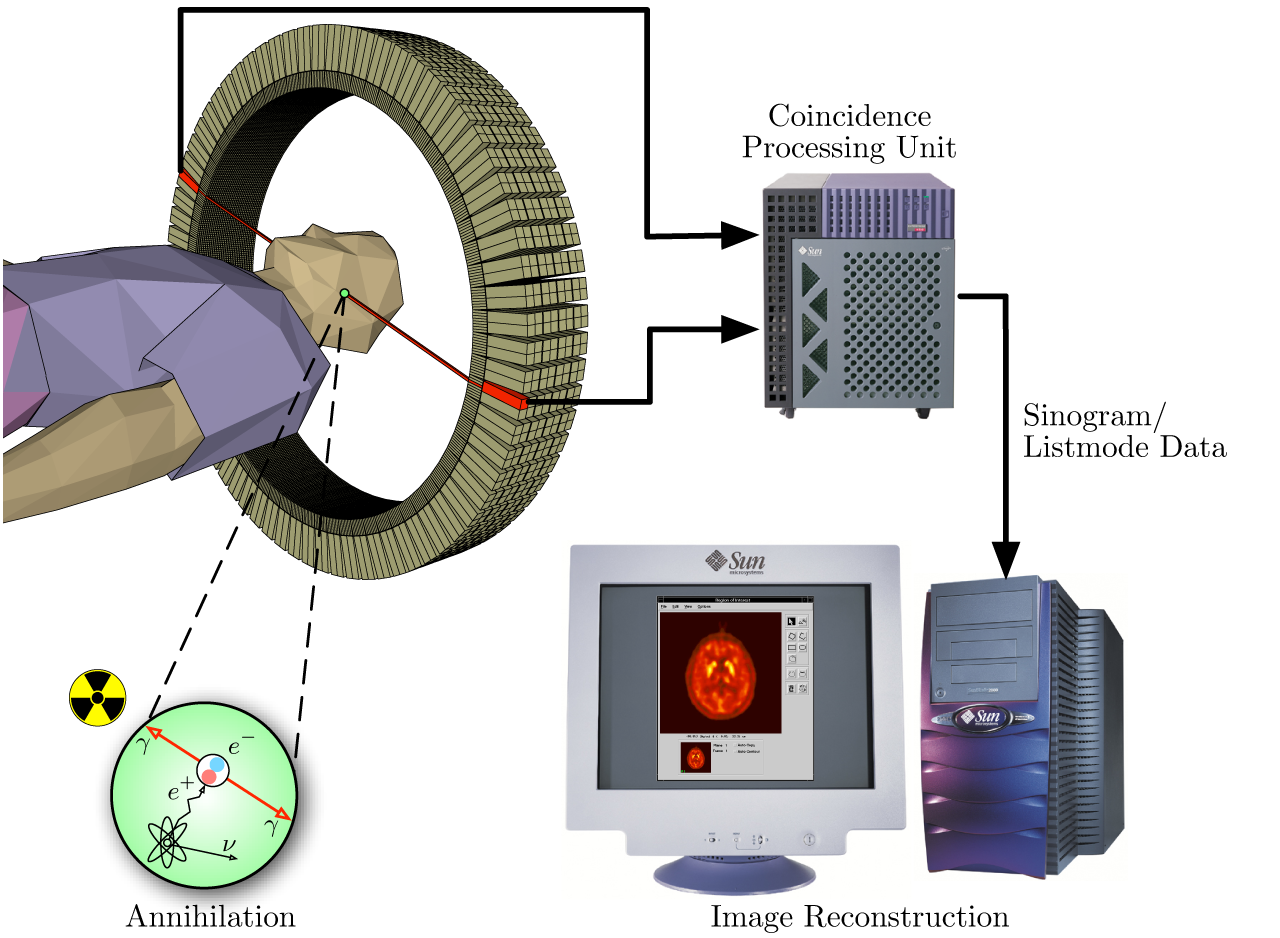
\includegraphics[scale=0.3]{../img/PET-schema.png}
	\caption{\label{fig.pet}: Principle of operation of PET. }
\end{figure}

\begin{figure}[!htb]
	\centering
	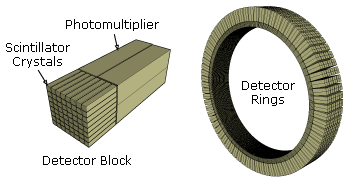
\includegraphics[scale=1.0]{../img/PET-detectorsystem_2.png}
	\caption{\label{fig.det}: A PET ring made of segmented solid scintillators. }
\end{figure}

The principle of operation (Figure \ref{fig.pet}) relies in injecting into the patient a  
biologically active molecule doped with a radioactive isotope, called tracer (a standard tracer is FDG, formed substituting an atom of oxygen by the isotope \FDG\ in a glucose molecule). The radionuclide decays and the resulting positrons
subsequently annihilate with electrons after traveling a short distance within the subject.
Each annihilation produces two 511 keV photons emitted most of the time in opposite
directions and these photons are registered by a detection system. The signal of each photon
from every pair coincidence event is processed individually for spatial, energy, and arrival
time information. For a pair coincidence event, if the energy of two photons stays within a
preset energy window, of the order of 20--30\% full-width-half-maximum (FWHM) for commercial systems, centered on the 511keV photopeak, and the timing difference stays within a preset time window (typically of up to some 10 ns), a
coincidence event will be registered and constitutes a line-of-response (LOR) for image
reconstruction.

In this paper we propose a (Positron Electron TOF Apparatus based on Liquid xenOn), {\bf PETALO}. The system is based in a very homogenous and compact detection cell (the Liquid Xenon Scintillating Cell, or LXSC), which captures with high efficiency the copious scintillation light produced in liquid xenon (LXe) as a response to the interaction of a 511 keV gamma.  the LXSC is readout by SiPMs connected to specialized ASICs optimized for excellent timing resolution. The high yield available in LXe, coupled to the fact that cryogenic operation of SiPMs eliminates the leading source of electronic noise in this devices (dark current) guarantees good energy and spatial resolution, while the fast scintillation time of LXe, combined with the homogeneity of the cell, guarantees a very low intrinsic CRT.

This paper is organised as follows. In section \ref{sec.det} we review the properties of the detectors used for PET scanners. In section \ref{sec.signalAndNoise} we describe signal and noise in PET reconstruction. In section \ref{sec.performance} we discuss the factors that determine the performance of PET scanners. In section \ref{sec.LXe} we review the relevant properties of liquid xenon as scintillating material. In section \ref{sec.petalo} we describe the characteristics and features of the PETALO concept. In section \ref{sec.conclu} we conclude. 

\section{Detectors used for PET scanners}
\label{sec.det}

The physical properties that define a detector suitable for a PET scanner are: 
{\bf Attenuation length ($\lambda$)}, which sets the scale of the length (across the photon line of flight) that the detector has to have in order to stop most of the incoming radiation.
{\bf Density ($\rho$)}, which is related with the total size and weight of the detector.
{\bf Photon yield per keV ($Y$)}, which must be as high as possible to record large signals. 
{\bf Refraction index ($r$)}, which must be as close as possible to the refraction index of photodetectors (glass in case of PMTs, $Si_3N_4$~ and $SiO_2$ layers for passivation and protection in case of semiconductor devices such as APDs and SiPMs). 
{\bf Energy resolution at 511 keV ($\sigma_E$)}, which must be as good as possible. 
{\bf Transverse spatial resolution ($\sigma_T$)} (relative to the photon line of flight), which in turn depends on the photon yield and the granularity of the readout sensors.
{\bf Longitudinal spatial resolution ($\sigma_L$)}, important to minimize the so-called parallax error and crucial to achieve a good coincidence resolving time (CRT).   
{\bf Scintillation decay time ($\tau$)}, which must be as short a possible, to maximize the number of events acquired per unit time and to minimize the window used to correlate events in different crystals. In addition, if the system has very good time resolution (in the range of few hundred picoseconds) time-of-flight measurements (TOF) are possible. 

Most modern PETs are built as rings using monolithic or segmented solid scintillating detectors read out by light sensitive detectors such as photomultipliers (PMTs), or silicon photomultipliers (SiPMs) (Figure \ref{fig.det}). Many of the high-end scanners use lutetium oxyorthosilicate (LSO)\footnote{LYSO (or lutetium-yttrium oxyorthosilicate) is also widely used. Both materials are very similar. In the rest of this document we will refer, for definiteness, to LSO.}, which is characterized by an {\bf attenuation length of 12 mm} to 511 keV photons, a  {\bf light yield of 26 photons per keV}, and a {\bf scintillation decay time of 40 ns}. This three parameters, essential for the performance of a PET scanner, result in an {\bf energy resolution} of typically 10-15 \% FWHM; a {\bf spatial resolution} of the order of 2-3 mm FWHM for the transverse coordinates. This is often achieved using segmented detectors read out by SiPMs. For example, for detectors of $3 \times 3$~mm$^2$~cross section, the rms resolution in the transverse coordinates is $\sim 3/\sqrt{12}$~mm, or about 2 mm FWHM. The error in 
the longitudinal coordinate goes as $\sim t/\sqrt{12}$, where $t$~ is the detector thickness. For $t \sim 20$~mm (enough to stop around 80\% of the incoming gammas), the rms error is 5.8 mm (13.3 mm FWHM). Finally, the {\bf coincidence resolving time} CRT measured in the laboratory is of the order of 200 ps (for systems at ambient temperature) and 500-600 ps for commercial devices.

\section{Signal and noise in PET reconstruction}
\label{sec.signalAndNoise}

\begin{figure}[!bthp]
	\centering
	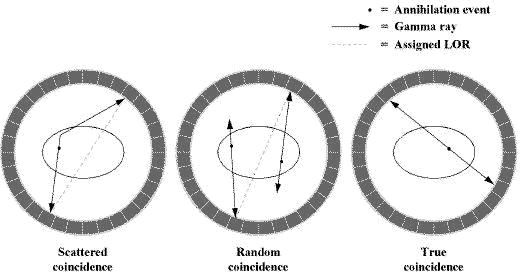
\includegraphics[scale=0.9]{../img/MAPD_coincidencecategories.jpg}
	\caption{\label{fig.coi} Coincidence detection principle in a PET detector.}
\end{figure}

The reconstruction of the image in a PET system requires crossing many LORs which in turn define one emission point in the area under study. LORs are formed by detecting the coincidence of two photons. Three types of coincidences, illustrated in Fig.~\ref{fig.coi}, are relevant:

\begin{itemize}
\item {\bf True coincidences} occur when both photons from an annihilation event are detected by detectors, neither photon undergoes any form of interaction prior to detection, and no other event is detected within the coincidence time-window.
\item {\bf A scattered coincidence} is one in which one of the detected photons (sometimes both) has undergone at least one Compton scattering event prior to detection. Since the direction of the photon changes due to the scattering process, the resulting coincidence event will, most likely, produce a wrong LOR. Scattered coincidences add a background to the true coincidence distribution which changes slowly with position, decreasing contrast and causing the isotope concentrations to be overestimated. They also add statistical noise to the signal. The number of scattered events detected depends on the volume and attenuation characteristics of the tissue being imaged. The best way to reject scattered coincidences is to build a PET system based on detectors with excellent energy resolution, since the scattered photons have also lost a fraction of their energy, and can therefore be rejected by imposing that the measured energy is inside a narrow window around 511 keV.
\item {\bf Random coincidences} occur when two photons, not arising from the same annihilation event, impinge the detectors within the coincidence time window of the system. As with scattered events, the number of random coincidences detected also depends on the volume and attenuation characteristics of the object being imaged, and on the geometry of the camera. The distribution of random coincidences is fairly uniform across the field of view and will cause isotope concentrations to be overestimated if not corrected for. Random coincidences also add statistical noise to the data. The best way to reject random coincidences is to build a PET system based on detectors with excellent CRT, since in this case one can impose a very narrow coincidence window. 
\end{itemize}

 A widely used
metric, reflecting the signal-to-noise ratio (SNR) performance of PET data in the context of
the three types of coincidences, is noise equivalent counts (NEC) defined as: 
%
\begin{equation}
NEC = \frac{T^2}{T+S+kR}
\label{eq.neq}
\end{equation}

Where T, S, and R are the total number of true, scattered and random coincidences,
respectively and k is a number between 1 and 2, depending on the phantoms/organs being imaged
and the random estimation methods being used. A higher NEC at a given injection dose
implies that a PET system is able to achieve better SNR and contrast-to-noise ratio (CNR)
performance.

\section{Performance of PET scanners}
\label{sec.performance}

The main goal of PET studies is to obtain a good quality and detailed image of an object. The critical parameters to achieve that goal are: i) a high photon detection sensitivity; ii) excellent spatial resolution, both in the transverse coordinates with respect to the gammas line of flight and in the coordinate along the gamma line of flight (depth of interaction or DOI) and iii) time of flight information, which requires excellent CRT. 

\subsection*{Photon detection sensitivity}

The photon detection sensitivity (often simply referred to as ``the sensitivity'') of a PET scanner is defined as the number of counts per unit time detected by the device for each unit of activity present in a source. It is normally expressed in counts per second per microcurie (or kilobecquerel) (cps/$\mu$Ci or cps/kBq). 
Assuming that dead time is small, sensitivity depends on the 
{\bf geometric efficiency (E$_g$)}, which defines the solid angle coverage of the detection system, and the {\bf intrinsic coincidence detection efficiency (E$_i$)},
which is determined by the detector atomic
number (Z), density, thickness of the detector along the path of the 511 keV gammas crystal, packing fraction, and the detector capability to set narrow windows for time and energy coincidence. The overall system
photon sensitivity (E$_s$) is simply the product of E$_g$~and E$_i$:

%
\begin{equation}
E_s = E_g \times E_i
\label{eq.gsensi}
\end{equation}

The photon sensitivity is often quoted for a
point positron source placed at the system center. In this particular case, the sensitivity can be expressed by the simple formula:

\begin{equation}
S = \frac{A \cdot \epsilon^2 \cdot e^{-\mu t} \cdot \xi}{4 \pi r^2} (\mathrm{cps}/\mu \mathrm{Ci})
\label{eq.sensi}
\end{equation}
%
where $\xi = 3.7 \times 10^4$~is a numerical conversion factor, $A$~is the detector area seen by the point source to be imaged, $\epsilon$~is the detector efficiency (e.g., the fraction of the time the detector is alive, which in turn depends on the detector scintillating time and the response of sensors, multiplied by the fraction of events that are relevant for detection, such as photoelectric interactions), $\mu$~is the linear attenuation coefficient of 511 keV photons in the detector material, $t$~is the detector thickness. Notice that the factor $\epsilon^2$~comes from the need to form a coincidence with two detectors with efficiency $\epsilon$. For an extended source at the center of such scanners, it has been shown that the geometric efficiency is approximated as w/2r, where w is the axial width of the detector element and r is the radius of the ring. Thus, the sensitivity of a scanner is highest at the center of the axial field-of-view (FOV) and gradually decreases toward the periphery.
For a standard clinical whole body PET
system, with 700--800 mm diameter bore, E$_s \sim 1$\%; for a typical
small animal PET system scanner (100--200 mm diameter bore), E$_s \sim 1-10$\%.

As can be seen in Eq.~\ref{eq.sensi}, the geometrical efficiency E$_g$ depends on the total solid angle of a PET system.  The most straightforward way to extend the solid angle is to increase the system
coverage along the axial field of view, that is, add new rings to the scanner. Unfortunately the detectors used today for such PET systems are expensive.

Consider for example a torso PET scanner with a diameter of 800 mm, and LSO detectors units of dimensions 5$\times$ 5 $\times $2 cm$^3$. A ring would require 50 detector units, and the cost of each unit (just the LSO detector, without including the readout and electronics) is about 2,500 \euro. Thus, the detectors to build a single ring cost 125 k\euro. The axial coverage is very modest (5 cm). Typical commercial systems feature an axial coverage around 20 cm, thus 4 rings are needed,  adding up to 0.5 M\euro\ just to pay the LSO detectors. Increasing the axial coverage to ``full torso'' (e.g., 50 cm) would require 1.25 M\euro\ to buy the LSO detectors, while the cost of the detectors for a ``full body'' scanner (e.g., 150 cm) would soar up to 3.75 M\euro\ . It follows that, {\em in order to increase axial coverage, and thus geometrical efficiency, the cost of the detector material must be as low as possible}.

There are several ways to increase $E_i$.
The most straightforward way is to use scintillation
materials with high Z and density, and thus the success of LSO, which features a density of 7.4 g/cm$^3$, and an attenuation length of only 12 mm. Materials of lower Z can in principle be used, provided that the detectors are made thicker. Increasing the length of crystals, however, results, as we have discussed, in a worsening of the DOI resolution and therefore in parallax errors when forming the LORs. In solid scintillators, thicker detectors also result in reduced light signal. 

$E_i$ can also be improved by tight packing of the crystals. In the example that we are discussing, the ideal packing would require to design crystals with the shape of a truncated pyramid. The entry face would have dimensions of $50 \times 50$~mm$^3$, while the exit face would have dimensions of $53 \times 53$~mm$^3$. Unfortunately, manufacturing block detectors with such shapes complicates the fabrication process and increases the cost of the system even further. 

Last, but not least, $E_i$~depends also on the coincidence time, which is typically set to 2 times the CRT, and on the energy window ($\sim 2\times$ energy resolution at 511 keV photopeak). In general, if the
other conditions remain the same, a system that exhibits better energy resolution and time
resolution will have a larger $E_i$.

To summarize, the requirements to achieve high photon sensitivity are:
\begin{enumerate}
\item Large axial coverage, which in turn requires low cost of the detection material per detection unit. 
\item Detectors with a short attenuation length for 511 keV gammas (which implies high density and hight Z), or, otherwise, capable to compensate with increased thickness a longer attenuation length. This requires that the DOI resolution does not degrade too much with thickness. 
\item Good energy resolution (which in turn requires high light yield) and good CRT (which requires fast scintillation).
\end{enumerate}

\subsection*{Spatial resolution of the PET system}

\begin{figure}[!bthp]
	\centering
	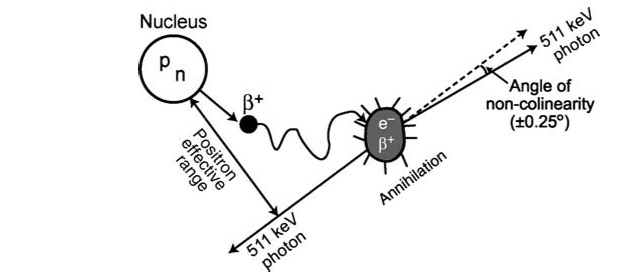
\includegraphics[scale=1.0]{../img/range.png}
	\caption{\label{fig.range} Positrons travel a distance before annihilation in the absorber and the distance increases with positron energy. Since positrons with different energies travel in zigzag directions, the effective range is the shortest distance between the nucleus and the direction of 511 keV photons. This effective range degrades the spatial resolution of the PET scanner.}
\end{figure}

The spatial resolution of a PET scanner is a measure of the ability of the device to faithfully reproduce the image of an object. It is empirically defined as the minimum distance between two points in an image that can be detected by the scanner. A number of factors contribute to the spatial resolution of the whole system.
\begin{itemize}
\item {\bf Individual detector resolution}: the scanner spatial resolution depends on the spatial resolution of the individual detectors used to build the system. As already discussed, conventional detectors such as LSO crystals do not measure, in general, the DOI.   
\item {\bf Positron range}: the emitted positron travels a distance in tissue, losing most of its energy by interaction with atomic electrons and then is annihilated after capturing an electron. Thus, the site of emission differs from the site of annihilation, as shown in Fig.~\ref{fig.range}. The distance (range) traveled by the positron increases with its energy, but decreases with the tissue density. Since the positrons are deflected after interaction with electrons resulting in a zigzag trajectory, the positron range is essentially an effective range, which is given by the shortest (perpendicular) distance from the emitting nucleus to the positron annihilation line. Furthermore, positrons are emitted with a distribution of energy, which also affects the effective range. The effective positron ranges in water for \ensuremath{^{18}}F is 2.2 mm. Since coincidence detection is related to the location of annihilation and not to the location of the positron emission, an error  occurs in the localization of true position of the positron emission thus resulting in the degradation of spatial resolution. However, this contribution to the spatial resolution is small, of the order of 0.2 mm for \ensuremath{^{18}}F.
\item {\bf Noncollinearity}: another factor of concern is the noncollinearity that arises from the deviation of the two annihilation photons from the fact that the two 511 keV photons are not emitted at exactly 180$^\circ$ after the annihilation process because of some small residual momentum of the positron at the end of the positron range. The maximum deviation from the 180$^\circ$ direction is $\pm 0.25^\circ$. Thus, the observed LOR between the two detectors does not intersect the point of annihilation, but is somewhat displaced from it. This error  degrades the spatial resolution of the scanner and deteriorates with the distance between the two detectors that register the photons. The contribution from noncollinearity worsens with larger diameters of the ring, and it amounts to 1.8--2 mm for currently available 80--90 cm PET scanners.
\end{itemize}

A relevant fact to take into account when designing a PET scanner is the intrinsic limitation introduced by the noncollinearity effect, which in turn sets the scale for the detector resolution. Since errors add quadratically, a detector resolution much smaller than the resolution introduced by noncollinearity does not bring any substantial benefit to the system. Thus, while small 10--20 cm scanners such as small animal PETs can aim for detector sub-mm resolution, the detector resolution of a large system does not need to be much better than 1--2 mm. 

\subsection*{Time of flight (TOF) application in a PET scanner}

\begin{figure}[!bthp]
	\centering
	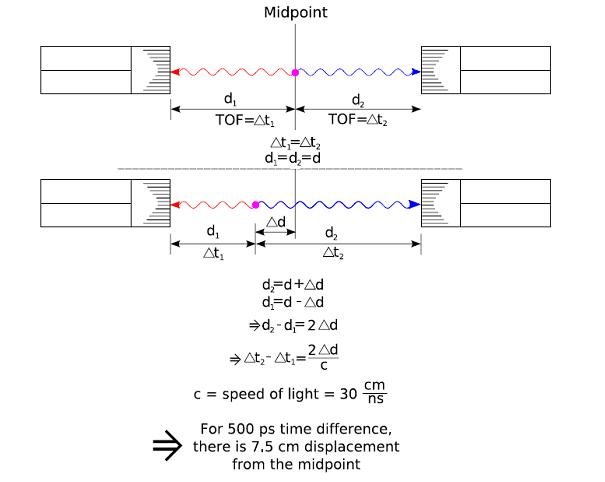
\includegraphics[scale=0.8]{../img/MAPD_tofprinciple.jpg}
	\caption{\label{fig.tof} Time of flight (TOF) principle in a PET detector.}
\end{figure}

A time-of-flight (TOF) PET scanner takes advantage of the difference in arrival times of two photons from the same annihilation event to infer spatial information of this event. 

To understand the principle of TOF applied to PET is important to recall that light in vacuum travels 30 cm in 1 ns. Consider the situation illustrated in Fig.~\ref{fig.tof}. In principle one can measure the point of emission along the LOR by taking the time of flight difference between the arrival of the two photons. Since:
\begin{equation}
\Delta t = \Delta t_2 - \Delta t_1 = \frac{2 \Delta d}{c}
\end{equation}
%
and $c$ = 30 cm/ns, it follows that the displacement from the mid point
$\Delta d$ is related with the TOF difference between the two photons $\Delta t$ and the speed of light $c$ as:

\begin{equation}
\Delta d =c \frac{2 \Delta t}{2}
\end{equation}

Thus, if one is able to measure $\Delta t$~ to a resolution of 500 ps (corresponding to the
best time resolution achieved by current commercial systems), the resulting precision in the
determination of $\Delta x$~is 7.5 cm, to be compared with the typical resolution achieved by
conventional PET, which is of the order of a few mm. A $\Delta t$~resolution of 25 ps would yield a resolution of better than 4 mm, competitive with that achieved in conventional PET scanner, and therefore TOF could be used to determine directly the emission point. 

\begin{figure}[!bhtp]
	\centering
	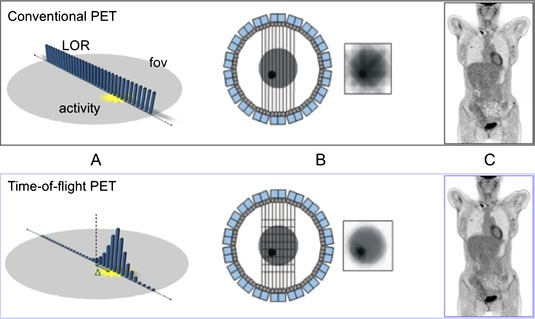
\includegraphics[scale=5]{../img/TOFPET.jpg}
	\caption{\label{fig.tile} TOF versus conventional PET. }
\end{figure}

%\begin{figure}[!bhtp]
%	\centering
%	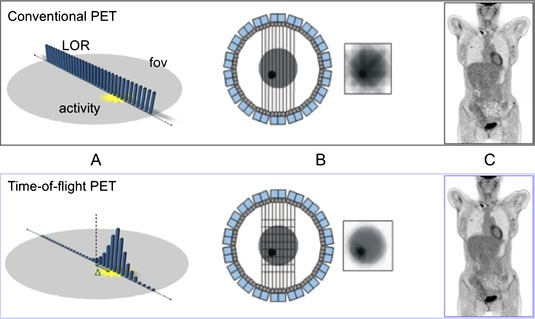
\includegraphics[scale=6]{../img/TOFPET.jpg}
%	\caption{\label{fig.tile} (A) Emission point at a distance d from the center of the scanner within an object of diameter D. The two 511 keV photons are detected in coincidence at times t1 and t2. (B) Without precise TOF measurement a uniform probability along the LOR within the object is assumed for each emission point, leading to noise correlations over a portion of image space between the two events as shown in (B). (C) With TOF information the position of the emission point is localized along the LOR with a precision that is defined by a Gaussian distribution of width $\Delta x$. (D) Better localization of the two emission events along their individual LORs leads to reduced noise correlation of the events in image space image reconstruction. }
%\end{figure}

In a TOF-PET scanner one uses good time-of-flight resolution to reduce the number of random coincidences, as illustrated in Fig.~\ref{fig.tile}. The principle is as follows. In a conventional PET without TOF one does not localize the emission point along the LOR. By collecting all possible LORs around the object (full angular coverage) and assuming uniform probability of the emission points lying along the full length of the LORs (and within object boundary), it is mathematically possible to reconstruct the emission object accurately. The knowledge of the emission point locations along the LORs is not necessary to reconstruct the emission object. However, by assuming uniform probability of event location along the full LOR length, noise from different emission events gets forward and back projected during image reconstruction over many image voxels leading to increased noise correlation. Hence, the image signal-to-noise ratio (SNR) gets reduced.

In TOF-PET the difference in the arrival times $(t_2 - t_1)$ of the two photons is measured with a precision $\Delta t$~(called coincidence resolving time, CRT) that helps localize the emission point along the LOR within a small region of the object. The uncertainty in this localization is determined by the CRT. The corresponding uncertainty in spatial localization $\Delta x$~ along the LOR is given by 
$\Delta x=c \times \Delta t/2$. As previously noted, if $\Delta x$~ is the same or smaller than the detector spatial resolution, then in principle image reconstruction is not needed. Typically this spatial localization, however, is more than one order of magnitude worse than the detector spatial resolution, and hence image reconstruction is still necessary to produce tomographic images. However, during reconstruction, noise from different events is now forward and back projected over only a limited number of image voxels as defined by the spatial uncertainty, leading to reduced noise correlations and improved image signal-to-noise resolution.
%  as illustrated in  Fig.~\ref{fig.tile}, panel D.
%
%
%\begin{figure}[!bhtp]
%	\centering
%	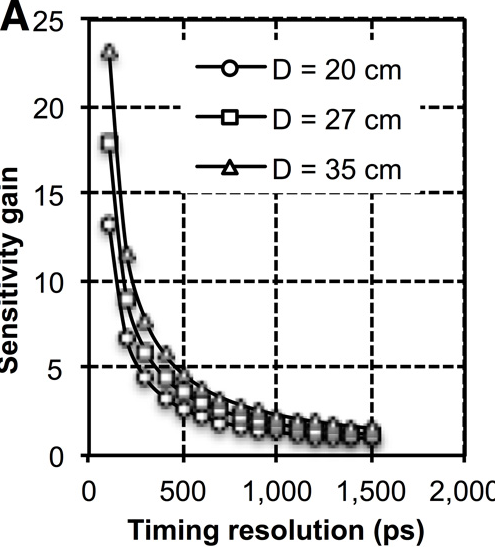
\includegraphics[scale=0.5]{img/SensiTof.png}
%	\caption{\label{fig.sensi} Gain in sensitivity (defined in the text) as defined by $D/\Delta x$ plotted as a function of timing resolution for cylindrical ``phantoms'' with three different diameters.}
%\end{figure}

With the knowledge that during the forward and back projection steps in image reconstruction noise will be spread over fewer voxels along the LOR (defined by $\Delta x$), it has been  shown  that the effective gain in sensitivity at the center of a uniform cylinder due to TOF information is given by $D/\Delta x$ \cite{snyder, budinger}. 
%Fig.~\ref{fig.sensi} shows a plot of this gain in sensitivity plotted as a function of timing resolution and for varying object sizes. As the object size increases or timing resolution improves, the gain due to TOF-PET increases. 

Consider as an example that one is performing a torso scan, ($D \sim 30$~cm). A PET capable of a CRT of 200 ps will result in $\Delta x = 3$~ cm and thus the gain in sensitivity may be as high as $30/3 = 10$). 
  
It follows that a PET scanner capable of a CRT in the range of 100 ps can improve the sensitivity by roughly a factor 10 w.r.t. a conventional PET with no TOF measurement. 


\subsection*{Summary: main requirements for a PET scanner}

From the discussion above we can conclude that the 
main requirements for a PET scanner are: 

\begin{enumerate}
\item {\bf Dense detectors}, with high stopping power for 511 keV gammas.
\item {\bf Spatial resolution of sub mm to few mm}, depending on the application (small animal PET requires sub mm resolution while full body PET can be done with a resolution of few mm).
\item {\bf Energy resolution as good as possible}, to eliminate Compton coincidences.
\item {\bf High count rate capability ($\sim10^6$ s$^{-1}$ cm$^{-2}$~ of detecting surface)}, which results in minimizing scan times and/or doses.
\item {\bf Fast scintillating time}, which allows narrow CRT and TOF applications. 
\item {\bf Large angular acceptance}, for torso, ``full body PET'', which in turn requires a large axial (along the patient's body) coverage. This requires cheap detection systems. 
\end{enumerate}


\section{Liquid xenon as detection material}\label{sec.LXe}

%
%\begin{figure}[!bhtp]
%	\centering
%	\includegraphics[scale=0.5]{img/XeLight.pdf}
%	\caption{\label{fig.xe} Signals in xenon.}
%\end{figure}

Xenon is a noble gas. It responds to the interaction of ionizing radiation providing both ionization and scintillation signals. The ionization signal is due to atomic electrons ejected from the xenon atoms by the incoming radiation, which take a long time to recombine due to the noble-gas nature of xenon (and therefore can be drifted to a collection electrode, if so desired). The scintillation signal is due to the de-excitation of xenon atoms forming dimers which decay after 2.2 ns (single mode) or 27 ns (triplet mode) emitting ultraviolet light (VUV) of 178 nm wavelength.

In its liquid phase (at a temperature of 165 K and atmospheric pressure) LXe has a reasonable high density (3 g/cm$^3$) and an acceptable attenuation length (30 mm), which makes it suitable for PET applications, in particular given the fact that one can compensate for the relatively large attenuation length by building thicker detectors while at the same time keeping an excellent resolution in the determination of the DOI. Compare with LSO, LXe offers:
\begin{enumerate}
\item {\bf A very high yield (60 photons per keV or about 30,000 photons for a 511 keV gamma)}, twice as large as that of LSO. Such a high yield translates into a small resolution error due to photon statistics which contributes to a good energy resolution, of the same order of that measured in LSO crystals, as discussed later. The high yield also contributes to a good spatial resolution (of the order of 2 mm FWHM) with a more spare instrumentation than that needed in LSO. Last but not least, a considerable fraction of the emitted photons (of the order of 6,000--8,000) decay with a fast constant of 2.2 ns, making possible an excellent CRT and therefore a PET-TOF application. 
\item {\bf LXe is a continuous medium with uniform response}. The design of a compact system is much simpler, then, than when using solid detectors of fixed shape. It is also possible to provide a 3D measurement of the interaction point, and, thus, a high resolution measurement of the DOI. Furthermore, in LXe it is possible to identify Compton events depositing all its energy in the detector as separate-site interaction, due to the relatively large interaction length in xenon. This increases the sensitivity of the system, since those events can, in principle, be used for image reconstruction. 
\item {\bf The refraction index of LXe is 1.55 for VUV light and 1.4 for blue light, to be compared with 1.8 for LSO}. The lower refraction index increases the acceptance of the sensors (it is much better matched to the entry window of the SiPMs) and introduces a smaller correction in the determination of the photoelectrons time stamp. 
\item {\bf The temperature of LXe at atmospheric pressure (160 K or -113 C)} is hot enough as to permit a simple cryostat, as well as normal operation of the SiPMs and the ASIC electronics, but cold enough to reduce the dark current rate (DCR) of the SiPMs by a factor $\sim 2^{13}$, thus making it essentially negligible. 
\item {The cost} of LXe is 20\% of the cost of LSO per detector unit. 
 \end{enumerate}

The first idea of using a LXeTPC for PET was proposed in 1993 by Chepel \cite{chepelFirst}. 
%The proposed detector was a LXe multi-wire detector consisting of six ionisation cells, each formed by two parallel cathode plates with a multi-wire anode in the middle. 
%Subsequent R\&D is documented in \footnote{{\em Chepel, V. Y. et al.}, 1995, Nucl. Instrum. Methods A
%367, 58; {\em Chepel, V. Y. et al.}, 1994, Nucl. Instrum. Methods
%A349, 500; {\em Chepel, V. Y. et al.}, 1997, Nucl. Instrum. Methods A392, 427; {\em Chepel, V. Y. et al., 1999, IEEE Trans NS-46, 1038}; {\em Crespo, P. et al.}, 1998, IEEE Trans. NS-45, 56; {\em Crespo, P. et al.}, 2000, IEEE Trans, NS-47, 2119; {\em Lopes, M. I. et al.}, 1995, IEEE Trans. NS-42, 2298.; {\em Thers D.}, ``A Positron Emission Tomograph (PET)
%based on a liquid Xenon Time Projection Chamber and Microstructure Devices for Compton tracking'', in Workshop on LXe-PET Camera, Subatech, Nantes, France, October 2003; }. 
%{\bf All those devices were based in the exploration of the ionisation signal in LXe}. {\em However, the measurement of such signals introduces a severe constrain to the technique, given the slow drift time of electrons in LXe} (typically of the order of 2 mm/$\mu$s, for a drifting field of 
%1 KV/cm). Since $\lambda = 3$.6~cm the practical length of a LXe cell (along the photon line of flight) must be of 5 cm to contain 80 \% of the photons. This, in turn, implies drifting times of 25 $\mu$s, which limits the interaction rate that can be recorded by the cell to  
%$\sim10^5 s^{-1}$, and therefore imposes a low-rate PET with a limited range of applications. 
%
The possibility of building a LXe PET (with TOF capabilities), based on the excellent properties of LXe as scintillator, was first suggested by Lavoie in 1976 \cite{lavoie}, and the study of this type of PET was carried out by the Waseda group \cite{Doke1,Nishikido2,Nishikido1}. The Waseda prototype was based in LXe cells read out by VUV-sensitive PMTs. In those cells one of the sides was left instrumented. The relatively poor performance of the system can be attributed in part to the use of PMTs and in part to the partial lack of instrumentation which affected both the energy and the time resolution. In spite of this limitations 
%The PMTs, although sensitive to the VUV light emitted by xenon had low quantum efficiencies (in the range 5-25 \%), and their rather large size compared with the size of the cell ($18\times 18$~mm$^2$) introduced significant geometrical effects which were difficult to correct. As a result of the above effects combined the energy resolution was of the same order than that of conventional SSDs. The space resolution was rather good, in the range of 2-3 mm, but only in the central volume of the cell (a cube of 5 mm size), and deteriorated rapidly in the borders, due to the space corrections introduced by the (relatively) large PMTs. 
the CRT achieved in the central volume of the prototype was excellent, of the order of 260 ps, showing the enormous potential of the technology for PET application. 

\section{PETALO}\label{sec.petalo}

PETALO (Positron Electron TOF Apparatus base on Liquid xenOn) is a TOF--capable, high sensitivity, PET scanner based in the excellent scintillating properties of LXe and using as building block a new type of detection cell,  the LXSC\footnote{Liquid Xenon Scintillating Cell, patent number P201531239 August 31st, 2015 presented to OPEM (MINECO), CSIC/UV.}. The key idea is the capability of the LXSC to capture with high efficiency, minimal geometrical distortions and uniform response, most of the light produced by the scintillation of xenon, a condition \emph{sine qua non} to achieve good energy and space resolution. 

\begin{figure}[!htbp]
	\centering
	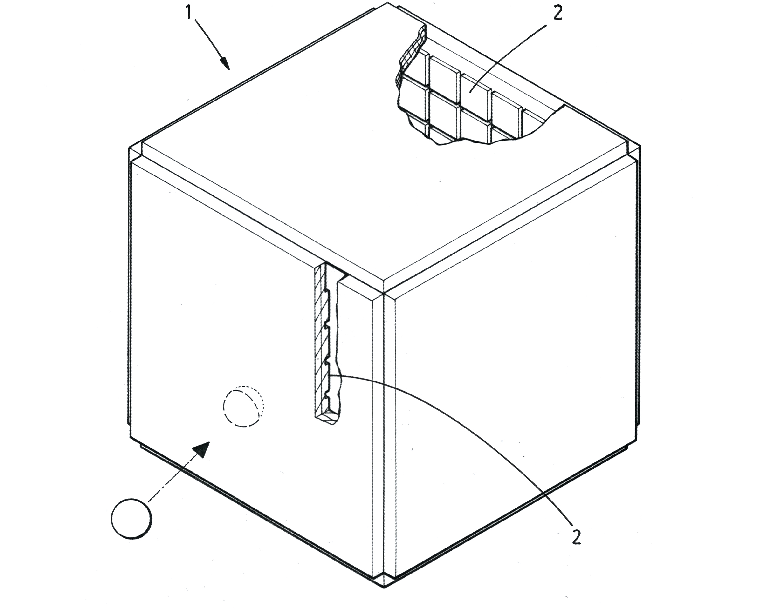
\includegraphics[scale=0.6]{../img/LXSC2.pdf}
	\caption{\label{fig.box} The Liquid Xenon Scintillating Cell (LXSC) instruments the entry and exit faces of the box (relative to the photon line of flight) with silicon photomultipliers (SiPMs), which can be eventually coated with a wavelength shifter, tetraphenyl butadiene (TPB). The non-instrumented faces are covered by reflecting Teflon (optionally also coated with TPB). The shape of the LXSC can be adapted to the application. }
\end{figure}

A drawing of the LXSC is shown in Fig.~\ref{fig.box}. In its simpler version is a box in which 
the entry and exit faces (relative to the photon line of flight) are instrumented with silicon photomultipliers (SiPMs), while the rest of the faces are covered with a highly reflective material such as teflon. The shape and the dimensions of the box itself can be adapted to the application. The size and type of SiPMs can also be tuned depending on the application.

For example, a scanner designed for large axial coverage (e.g, ``full body PET'') could be based on trapezoidal cells (to maximize the packing) of large transverse dimensions and a thickness of 5-6 cm (to stop $\sim$80\% of the incoming gammas). The cell could use large
SiPMs (e.g., 6 mm length) coated with a suitable wavelength shifter, such as tetraphenyl butadiene (TPB). The teflon panels covering the non-instrumented faces can also be coated with TPB. Notice that TPB shifts the VUV light (172 nm) emitted by the LXe  to wavelengths around 430 nm (where the PDE of conventional SiPMs is maximal) with an efficiency of better than 80\%. Furthermore, TPB does not absorb blue light above 400 nm, therefore minimizing losses. On the other hand, several manufacturers offer today SiPMs of large area, high gain, low dark current and very low noise which can operate at liquid xenon temperatures with excellent performance.

Instead, a scanner designed to optimize sensitivity, including excellent CRT (better than 100 ps, as described below), would use SiPMs optimized for spatial and time resolution. An attractive possibility are the Hamamatsu VUV MPPCs, with 3 mm size and sensitive to 172 nm light with a PDE of around 15\%. Such a scanner could represent a breakthrough if applied to brain imaging.  

An initial study of the expected performance of the LXSC defined above (called the LXSC2) has been conducted using Monte Carlo simulation\footnote{J.M. Benlloch Rodr\'iguez, {\bf PETALO, a new concept for a Positron Emission TOF apparatus based on liquid Xenon}, Master thesis, University of Valencia, September, 2015.}. We describe below some of the most significative results:

\subsection{Energy and spatial resolution}

\begin{figure}[!htb]
	\centering		
		\subfloat[LXSC2, $x$ coordinate]{
			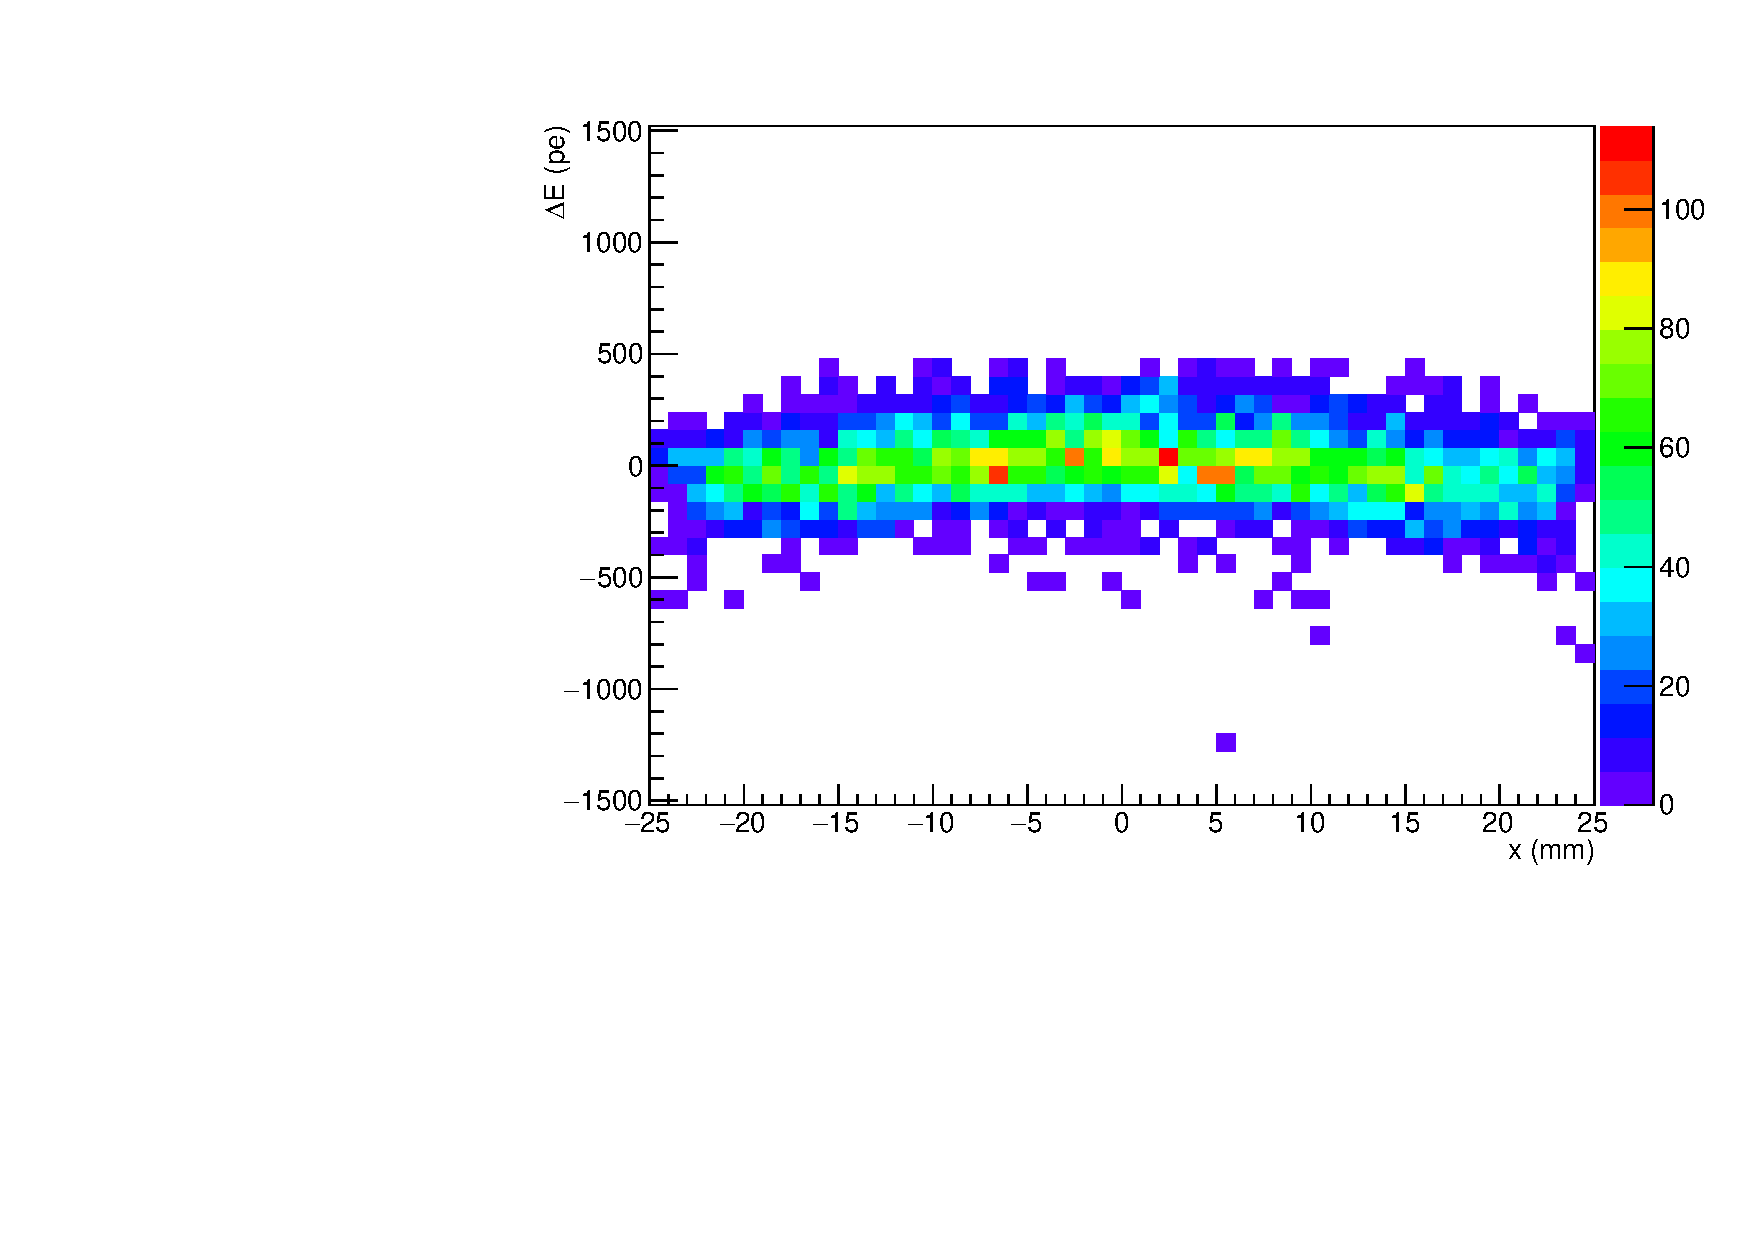
\includegraphics[width=.6\textwidth]{../img/eposx_264.pdf}
			\label{fig.eposx264}		}
		\subfloat[LXSC2, $z$ coordinate]{
			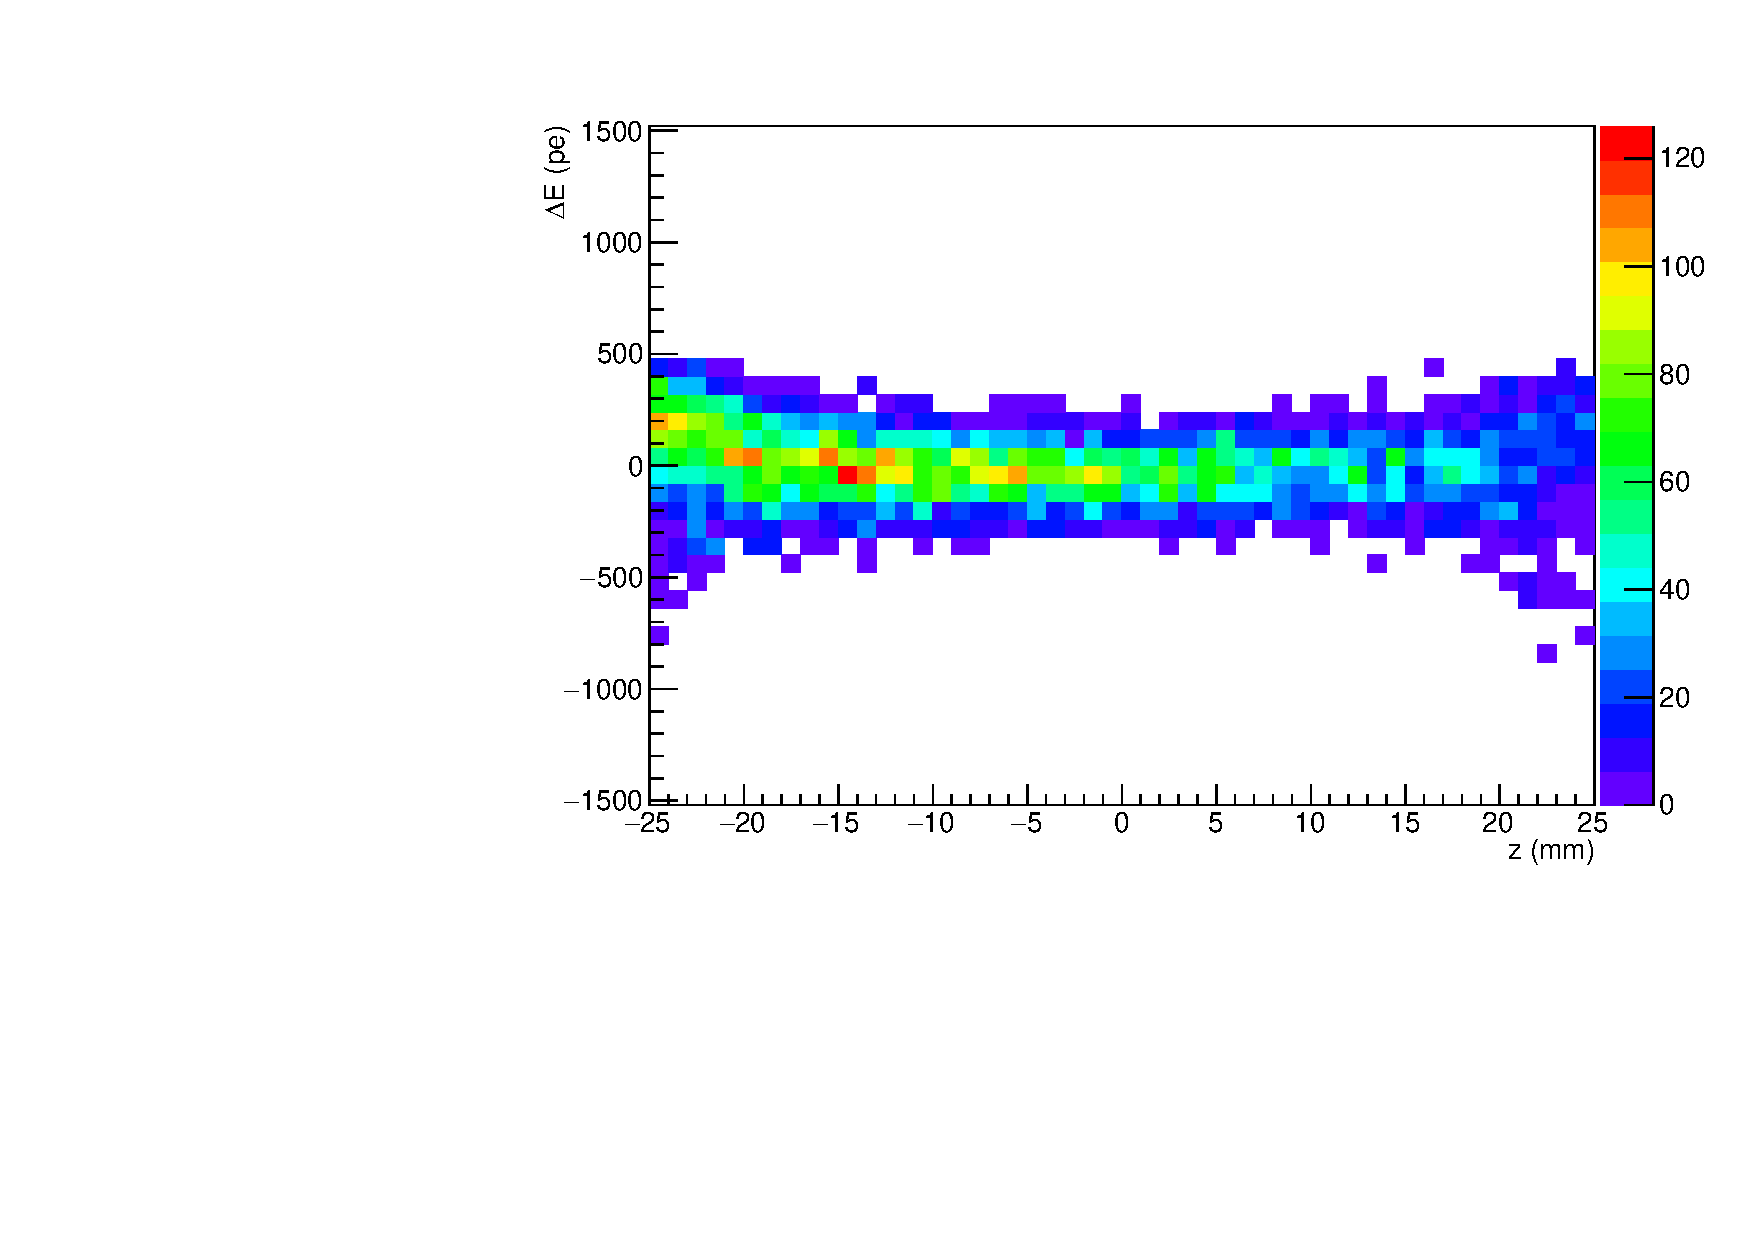
\includegraphics[width=.6\textwidth]{../img/eposz_264.pdf}
			\label{fig.eposz264}
		}
	\caption{\label{fig.energyDep2} Difference between the reconstructed energy and the average energy ($\Delta E$) as a function of one coordinate. (a) Energy dependence with the transverse coordinate ($x$) in LXSC2. (b) Energy dependence with the longitudinal coordinate ($z$) in LXSC2.}
\end{figure}


The energy resolution R of a liquid xenon scintillation detector is a combination of light collection variation due to the detector geometry R$_g$, the statistical fluctuation of number of photoelectrons from the sensors R$_s$, the fluctuation of electron-ion recombination due to escape electrons $R_r$, and the intrinsic resolution from liquid xenon scintillation light R$_i$, due to the non-proportionality of scintillation yield due to secondary electrons. Then:

\begin{equation}
R^2 = R_g^2 + R_s^2 + R_r^2 + R_i^2
\end{equation}

The contribution of the intrinsic terms, ($R_r$~and R$_i$) has been measured to be
around 11 \% FWHM \cite{aprileRes}. We have computed the contribution of photoelectron statistics and geometrical effects for a large
($5 \times 5 \times 5 {\rm ~cm^3}$) LXSC equipped with SiPM of 6 mm coated with TPB (the LXSC2).  
Figure \ref{fig.energyDep2} show the difference between reconstructed energy and average energy as a function of one of the transverse coordinates (x) and the longitudinal coordinate (z) defining the thickness of the LXSC. Notice that the dependence of the energy with the longitudinal and transverse coordinates is very soft, and will introduce a relatively minor effect in the energy resolution even if left uncorrected. An energy resolution of 3.0 \% FWHM due to the combined effect of photoelectron statistics and geometrical effect is obtained. 
An overall resolution of the order of 12\% FWHM, which is of the same order as that achieved with LSO detectors, is expected. 

The spatial resolution in the (x,y) coordinates (transverse to the gammas line of flight) is obtained by the weighted pulses in the SiPMs. The digital resolution would be
$p/\sqrt{12}$, where $p$~is the pitch. With a pitch of 6 mm (see methodology) we expect 1.7 mm rms or 4 mm FWHM. Weighting with the SiPM amplitude improves the resolution to about 2 mm FWHM. The longitudinal coordinate (along the gammas line of flight) is obtained by computing the ratio between the
total signal recorded in the entry and exit face, and is found to be also 2 mm FWHM. 


\subsection*{CRT  of the LXSC}

The intrinsic CRT of a LXe detector depends on two factors: a) the time resolution to trigger in interactions occurring in individual cells and b) the time jitter introduced by the synchronization of the individual triggers (singles) into a ``double'' involving two cells. 

The ``single'' time resolution, on the other hand, depends on: a) the ratio $N/\tau$, where $N$ is the number of photons emitted with a given time decay constant $\tau$; b) the DOI correction, which takes into account that not all the interactions in the cell occur in the same point; c) the SiPM PDE; d) the time jitter introduced by the SiPM and the associated electronics. 

The relevant figure of merit to evaluate the CRT of a scintillator producing $N$~photons with a decay constant $\tau$~is $\tau/\sqrt{N}$. For LXe, $\tau=2200$~ps, $N \sim 6000$, thus 
$\tau/\sqrt{N} \sim 28$~ps. For LSO, $\tau=40000$~ps, $N \sim 14000$, thus 
$\tau/\sqrt{N} \sim 338$~ps. The ratio between LXe and LSO is a factor 12. 
Furthermore, the capability to measure the DOI with very good resolution minimizes the jitter introduced by the DOI correction, which goes like
${\rm \Delta t = \Delta z}$(n - 1) 0.033 ns/cm, where $\Delta t$~ is the time resolution introduced by the resolution $\Delta z$ in the determination of the DOI $z$ and $n$~is the refraction index. In LXe, assuming a DOI resolution of 2 mm FWHM, and setting $n=1.6$ (for VUV light), one obtains $\Delta t \sim 4$~ps FWHM. In a conventional LSO crystal of 2 cm length, $\Delta t \sim 35$~ps FWHM.

The effect of the SiPMs needs to be carefully measured. The time jitter introduced by the SiPMs depends of its capacitance (thus it is better to use SiPMs of moderate size, e.g., 3 mm rather than 6 mm), the time constant of the SiPM signal, the PDE, etc. A detailed model of the SiPM can be constructed and incorporated into a simulation to predict the effect of the sensor in the CRT, and experimental measurements are needed to validate the model and to produce an estimation of the CRT that the technology can achieve. However, our initial simulations show that a CRT better than 80 ps can be achieved. 


\section{Summary and outlook}\label{sec.conclu}
We have presented PETALO, a PET scanner based in the LXSC, a compact, homogenous and highly efficient liquid xenon cell, which constitutes the apparatus building block. PETALO exploits the high yield and fast decay constant of LXe, to achieve good energy and spatial resolution and excellent CRT. Our Monte Carlo calculations show that an energy resolution of 12\% FWHM, an spatial resolution of 2 mm FWHM (in the three coordinates) and a CRT better than 80 ps can be achieved. 

The main application of PET to medicine is oncology. A typical dose of FDG used in an oncological scan has an effective radiation dose of 14 mSv, equivalent to about 5 years of dose by background radiation (combining natural and artificial sources). It follows that one of the important issues in PET applications is to reduce the FDG dose as much as possible, which, in turn requires an axial coverage as large as possible. Today's scanner have axial lengths of 15-25 cm. A larger scanner improves the solid angle, resulting in a larger acceptance and therefore allowing a dose reduction. Unfortunately, {\bf the cost of current PET scanners is very high}, limiting their dimensions, and in particular its axial length. The fact that  individual PET scans are more expensive than ``conventional'' imaging with computed tomography (CT) and magnetic resonance imaging (MRI) limits also their use in clinical diagnose. {\bf Reducing costs of PET scanners is, therefore, a major priority to facilitate the expansion of the technology}. Conversely, the combination of PET with CT and MRI often leads to much improved scans, since the structural information offered by CT and MRI can be combined with the functional information offered by PET. 

PET neuroimaging uses the fact that the brain is an avid user of glucose, and since brain pathologies such as Alzheimer's disease greatly decrease brain metabolism of glucose, standard FDG-PET of the brain, which measures regional glucose use, may also be successfully used to differentiate Alzheimer's disease from other dementing processes, and also to make early diagnosis of Alzheimer's disease. Neuroimaging requires images as clear as possible, and therefore high--performance PET scanners fully compatible with MRI (thus capable of operating in very intense, highly variable magnetic fields). Using time-of-flight (TOF) information is one of the best ways of boosting performance, insofar as the sensitivity of the scanner improves with $D/CTR$~, where $D$~is the diameter of the object being imaged (e.g., the head). An order of magnitude improvement in sensitivity can be reached by using a PETALO scanner with a CTR of 100 ps. 

A PETALO scanner intended as a large acceptance ``full body'' PET, of $\sim$ 150 cm axial length and some 60-80 cm diameter could be built stacking 30 rings, each one made of about 40 large cells of $5 \times 5 \times 5$~cm$^3$~with (relatively) sparse SiPM instrumentation (32 SiPM per face, for a total of 64 SiPM per LXSC). The scanner would have lower cost (due to the comparatively low cost of LXe, and the sparse instrumentation) and better sensitivity (due to the  improved CTR) than a LSO scanner.  

A PETALO scanner intended for neuroimaging can increase the number of SiPMs, reduce their size and implement VUV sensitive devices to optimize the energy resolution and the spatial resolution, while aiming to a  CTR  better than 80 ps. Such a device would be a true breakthrough with respect to the state-of-the-art in brain scanners. 

Last but not least, the PETALO technology is expected to be fully compatible with MRI, thus making it suitable for combined MRI-PET scanners. 


\section*{}

\bibliography{biblio.bib}

\end{document}